\documentclass[aspectratio=169]{beamer}

% Theme settings
\usetheme{Madrid}
\usecolortheme{Columbia}
\setbeamertemplate{navigation symbols}{}
\setbeamertemplate{itemize items}[circle]

% Packages
\usepackage{amsmath}
\usepackage{amssymb}
\usepackage{bm}
\usepackage{graphicx}
\usepackage{booktabs}
\usepackage[table]{xcolor}
\usepackage{tikz}
\usepackage{pgfplots}
\pgfplotsset{compat=1.18}
\usetikzlibrary{decorations.pathmorphing,patterns,arrows.meta,shapes,positioning}
\usepackage{hyperref}

% Title Information
\title[Regenerative Cooling \& FFSC]{Regenerative Nozzle Cooling \& Full-Flow Staged Combustion Cycles}
\subtitle{Modeling, Analysis, and Optimization}
\author{David Tew}
\institute{Columbia University}
\date{\today}

\begin{document}

%---------------------------------------------------------
% Title Slide
%---------------------------------------------------------
\begin{frame}
  \titlepage
\end{frame}

%---------------------------------------------------------
% Section 1: Introduction
%---------------------------------------------------------
\section{Introduction}

\begin{frame}{Lecture Overview}
  \begin{block}{Topics Covered}
    \begin{enumerate}
      \item Regenerative nozzle cooling fundamentals
      \item Full-flow staged combustion (FFSC) cycle architecture
      \item Governing equations for 1D cooling model
      \item Turbopump power balance
      \item Python implementation and optimization
      \item Example: $CH_4/LOX$ engine design
    \end{enumerate}
  \end{block}
  \vspace{0.5cm}
  \textbf{Goal:} Understand coupled thermal-fluid-cycle analysis of liquid rocket engines.
\end{frame}

\begin{frame}{Why Regenerative Cooling?}
  \begin{columns}
    \column{0.6\textwidth}
    \textbf{The Challenge:}
    \begin{itemize}
      \item Combustion gas temperature: $T_0 \approx 3600$ K ($CH_4$/$O_2$)
      \item Nozzle wall materials melt at $\sim$2000 K
      \item Film/ablative cooling inefficient for reusability
    \end{itemize}
    \vspace{0.3cm}
    \textbf{The Solution: Regenerative Cooling}
    \begin{itemize}
      \item Route cryogenic propellant through jacket around nozzle
      \item Convective heat transfer cools walls
      \item Heated propellant feeds combustion chamber
      \item Enables reusable, high-performance engines
    \end{itemize}

    \column{0.4\textwidth}
    \centering
    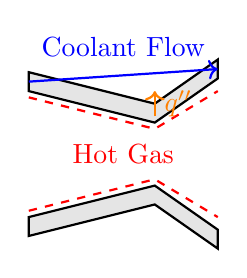
\begin{tikzpicture}[scale=0.8]
      % Nozzle wall
      \draw[thick,fill=gray!20] (0,1) -- (2,0.5) -- (3,1.2) -- (3,1.5) -- (2,0.8) -- (0,1.3) -- cycle;
      \draw[thick,fill=gray!20] (0,-1) -- (2,-0.5) -- (3,-1.2) -- (3,-1.5) -- (2,-0.8) -- (0,-1.3) -- cycle;
      
      % Hot gas
      \draw[thick,red,dashed] (0,0.9) -- (2,0.4) -- (3,1.0);
      \draw[thick,red,dashed] (0,-0.9) -- (2,-0.4) -- (3,-1.0);
      \node[red] at (1.5,0) {Hot Gas};
      
      % Cooling channels
      \draw[blue,thick,->] (0,1.15) -- (3,1.35);
      \node[blue,above] at (1.5,1.4) {Coolant Flow};
      
      % Heat flux arrows
      \draw[->,thick,orange] (2,0.6) -- (2,1.0);
      \node[orange,right] at (2,0.8) {$q''$};
    \end{tikzpicture}
  \end{columns}
\end{frame}

%---------------------------------------------------------
% Section 2: FFSC Cycle Architecture
%---------------------------------------------------------
\section{FFSC Cycle Architecture}

\begin{frame}{Full-Flow Staged Combustion (FFSC) Cycle}
  \textbf{Key Features:}
  \begin{itemize}
    \item \textit{All} propellant flows through preburners
    \item Two preburners: fuel-rich and ox-rich
    \item Turbines driven by preburner exhaust
    \item High chamber pressure capability
    \item Highest theoretical $I_{sp}$ of any cycle
  \end{itemize}
  \vspace{0.3cm}
  \textbf{Advantages:}
  \begin{itemize}
    \item No wasted propellant (vs. gas generator)
    \item Lower turbine temperatures than ox-rich SC
    \item Excellent for methane/LOX
  \end{itemize}
\end{frame}

\begin{frame}{FFSC Flow Split Strategy}
  \textbf{Propellant Distribution:}
  \begin{itemize}
    \item \textbf{Fuel side:}
    \begin{itemize}
      \item Large fraction ($\sim$95\%) routed through cooling jacket
      \item Remainder to fuel-rich preburner with small ox injection
      \item Preburner operates at $\phi \approx 1.3$ (fuel-rich)
    \end{itemize}
    \item \textbf{Oxidizer side:}
    \begin{itemize}
      \item Majority to ox-rich preburner with small fuel injection
      \item Preburner operates at $\phi \approx 0.7$ (ox-rich)
      \item Remainder injected directly to main chamber
    \end{itemize}
  \end{itemize}
  \vspace{0.4cm}
  \textbf{Design Constraint:}
  \begin{equation*}
    P_{\text{turb,avail}} \geq \frac{P_{\text{pump,req}}}{\eta_{\text{mech}}} \quad \text{(on each side)}
  \end{equation*}
\end{frame}

%---------------------------------------------------------
% Section 3: Governing Equations
%---------------------------------------------------------
\section{Governing Equations}

\begin{frame}{1D Nozzle Flow Model}
  \framesubtitle{Isentropic core flow with Bartz heat transfer}
  
  \textbf{Isentropic Relations:}
  \begin{align*}
    T(x) &= \frac{T_0}{1 + \frac{\gamma-1}{2}M(x)^2} \\
    p(x) &= p_0 \left(\frac{T(x)}{T_0}\right)^{\gamma/(\gamma-1)}
  \end{align*}
  
  \textbf{Bartz Gas-Side Heat Transfer Coefficient:}
  \begin{equation*}
    h_g = \frac{0.026}{D_t^{0.2}} \left( \frac{\mu^{0.2} C_p}{Pr^{0.6}} \right)_0 \left( \frac{P_c}{c^*} \right)^{0.8} \left( \frac{A_t}{A} \right)^{0.9} \sigma
  \end{equation*}
  
  \vspace{0.2cm}
  \centering
  \alert{$h_g$ highest at the throat due to high pressure and temperature.}
\end{frame}

\begin{frame}{Coolant-Side Heat Transfer}
  \framesubtitle{Turbulent internal flow with property variations}
  
  \textbf{Reynolds and Prandtl Numbers:}
  \begin{equation*}
    \text{Re} = \frac{G D_h}{\mu}, \quad \Pr = \frac{c_p \mu}{k}, \quad D_h = \frac{4A_c}{P_{\text{wet}}}
  \end{equation*}
  
  \textbf{Gnielinski Correlation (Re $>$ 2300):}
  \begin{equation*}
    \text{Nu} = \frac{(f/8)(\text{Re}-1000)\Pr}{1 + 12.7\sqrt{f/8}(\Pr^{2/3}-1)} \left(\frac{\mu_b}{\mu_w}\right)^{0.14}
  \end{equation*}
  
  \textbf{Coolant Heat Transfer Coefficient:}
  \begin{equation*}
    h_c = \frac{\text{Nu} \cdot k}{D_h}
  \end{equation*}
  
  \vspace{0.2cm}
  \centering
  Sieder-Tate correction accounts for viscosity variation near wall.
\end{frame}

\begin{frame}{Conjugate Heat Transfer}
  \framesubtitle{Series thermal resistances}
  
  \textbf{Total Thermal Resistance:}
  \begin{equation*}
    R_{\text{tot}} = \frac{1}{h_g} + \frac{t_{\text{wall}}}{k_{\text{wall}}} + \frac{1}{h_c}
  \end{equation*}
  
  \textbf{Heat Flux:}
  \begin{equation*}
    q''(x) = \frac{T_g(x) - T_{\text{cool}}(x)}{R_{\text{tot}}(x)}
  \end{equation*}
  
  \textbf{Inner Wall Temperature:}
  \begin{equation*}
    T_{\text{wall,inner}}(x) = T_g(x) - \frac{q''(x)}{h_g(x)}
  \end{equation*}
  
  \vspace{0.3cm}
  \textbf{Design Limit:} $T_{\text{wall,inner}} < T_{\text{melt}}$ or structural limit ($\sim$900 K for Inconel/Cu alloys)
\end{frame}

\begin{frame}{Coolant Energy Balance}
  \framesubtitle{Axial integration of coolant heating}
  
  \textbf{Energy Equation (Steady 1D):}
  \begin{equation*}
    \dot{m}_{\text{cool}} c_{p,c} \frac{dT_{\text{cool}}}{dx} = q''(x) P_{\text{inner}}(x)
  \end{equation*}
  
  \textbf{Discrete Form:}
  \begin{equation*}
    T_{\text{cool},i+1} = T_{\text{cool},i} + \frac{q''_i P_{\text{inner},i} \Delta x}{\dot{m}_{\text{cool}} c_{p,c,i}}
  \end{equation*}
  
  \vspace{0.3cm}
  \textbf{Coolant Pressure Drop (Darcy-Weisbach):}
  \begin{equation*}
    \Delta p_{\text{cool}} = f \frac{L}{D_h} \frac{\rho v^2}{2}
  \end{equation*}
  
  \small
  Integrated along nozzle to ensure $p_{\text{cool}} > p_0$ at all stations.
\end{frame}

\begin{frame}{Turbopump Power Balance}
  \framesubtitle{Ensure turbines can drive pumps}
  
  \textbf{Pump Power Required:}
  \begin{equation*}
    P_{\text{pump}} = \frac{\dot{m} \Delta p}{\rho \eta_{\text{pump}}}
  \end{equation*}
  
  \textbf{Turbine Power Available:}
  \begin{equation*}
    P_{\text{turb}} = \dot{m}_{\text{turb}} c_p (T_{\text{in}} - T_{\text{out}}) \eta_{\text{turb}}
  \end{equation*}
  
  \textbf{Feasibility Criterion (Each Side):}
  \begin{equation*}
    P_{\text{turb,avail}} \geq \frac{P_{\text{pump,req}}}{\eta_{\text{mech}}}
  \end{equation*}
  
  \vspace{0.3cm}
  \small
  Typical values: $\eta_{\text{pump}} \approx 0.75$, $\eta_{\text{turb}} \approx 0.90$, $\eta_{\text{mech}} \approx 0.98$
\end{frame}

%---------------------------------------------------------
% Section 4: Implementation & Results
%---------------------------------------------------------
\section{Implementation \& Results}

\begin{frame}{Python Model Implementation}
  \
  \textbf{Modular Structure:}
  \begin{itemize}
    \item \texttt{thermo}: Cantera equilibrium chemistry for chamber state
    \item \texttt{regen}: 1D regenerative cooling along nozzle contour
    \item \texttt{cycle}: Full FFSC power balance and feasibility check
    \item \texttt{sweep}: Parameter sweeps and optimization routines
  \end{itemize}
  
  \vspace{0.1cm}
  \textbf{Key Inputs:}
  \begin{itemize}
    \item Thrust $F_{\text{vac}}$, chamber pressure $p_0$, O/F ratio
    \item Nozzle geometry: throat radius $r_t$, expansion ratio $\varepsilon$
    \item Cooling parameters: channel count, dimensions, coolant fraction
    \item Turbomachinery efficiencies and preburner temperatures
  \end{itemize}
  
  \vspace{0.1cm}
  \textbf{Outputs:}
  \begin{itemize}
    \item Wall temperature profile, coolant heating and pressure drop
    \item Pump/turbine power requirements and margins
    \item FFSC cycle feasibility (fuel and ox sides)
    \item Mermaid flow diagram generation for visualization
  \end{itemize}
\end{frame}

\begin{frame}{FFSC "Mermaid" Schematic Diagram}
  \centering
  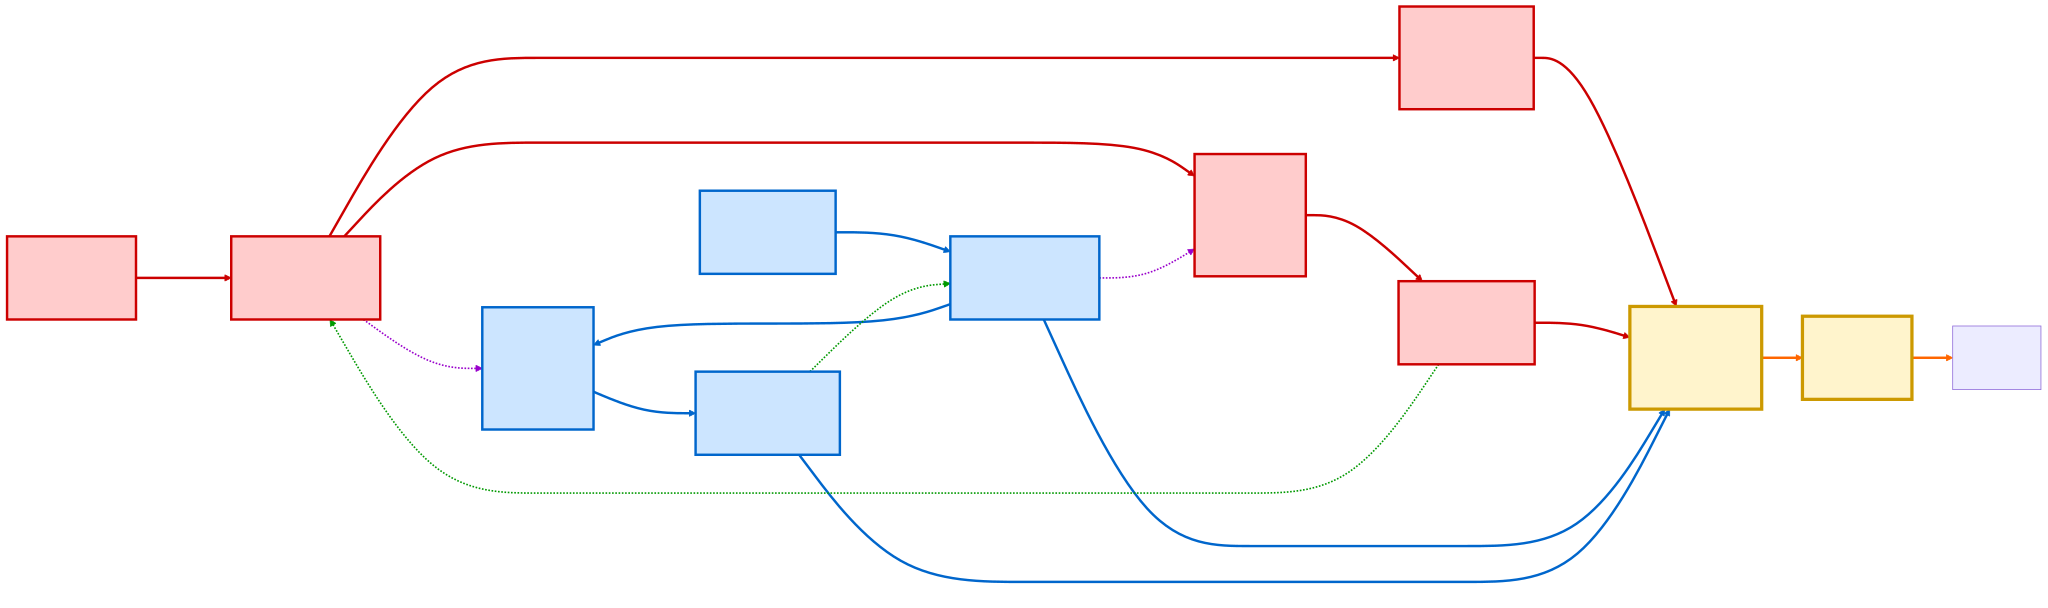
\includegraphics[width=\textwidth]{figs/mermaid_ffsc_diagram.png} \\
  \vspace{0.2cm}
  Schematic of FFSC cycle showing propellant flow paths and turbopump arrangement
\end{frame}

\begin{frame}{Example: 500 kN $CH_4/LOX$ Engine}
  \framesubtitle{Baseline design parameters}
  
  \begin{columns}
    \column{0.5\textwidth}
    \textbf{Design Parameters:}
    \begin{itemize}
      \item $F_{\text{vac}} = 500$ kN
      \item $p_0 = 20$ MPa
      \item $\text{O/F} = 3.2$
      \item $r_t = 0.10$ m
      \item $\varepsilon = 15$
      \item $L_{\text{noz}} = 1.2$ m
      \item $T_{\text{fuel,tank}} = 110$ K
      \item $T_{\text{ox,tank}} = 90$ K
    \end{itemize}
    
    \column{0.5\textwidth}
    \textbf{Cooling Configuration:}
    \begin{itemize}
      \item 300 channels
      \item Channel width: 3 mm
      \item Wall thickness: 1.5 mm
      \item $p_{\text{cool,in}} = 30$ MPa
      \item Coolant fraction: 95\% of fuel
    \end{itemize}
    \vspace{0.3cm}
    \textbf{Turbomachinery:}
    \begin{itemize}
      \item $T_{\text{turb,out}} = 1000$ K
      \item $\eta_{\text{pump}} = 0.75$
      \item $\eta_{\text{turb}} = 0.92$
    \end{itemize}
  \end{columns}
\end{frame}

\begin{frame}{Nozzle Cooling Results}
  \framesubtitle{Temperature and heat transfer coefficient profiles}
  
  \begin{columns}
    \column{0.45\textwidth}
    \textbf{Key Results:}
    \begin{itemize}
      \item \alert{$T_{\text{wall,max}} = 2000$ K}
      \item $\Delta p_{\text{cool}} = 2.5$ MPa
      \item $T_{\text{cool,out}} = 350$ K
      \item Peak heat flux at throat: $TBD$ MW/m²
    \end{itemize}
    \vspace{0.3cm}
    \textbf{Observations:}
    \begin{itemize}
      \item Wall temp peaks near throat
      \item Coolant heats rapidly in throat region
      \item Gas-side HTC dominates thermal resistance
      \item Pressure drop manageable ($<$10\% of inlet)
      \item Design satisfies thermal limits
    \end{itemize}
    
    \column{0.55\textwidth}
    \centering
    \includegraphics[width=0.75\textwidth]{figs/regen_nozzle_cooling.png}
    \vspace{0.2cm}
  \end{columns}
\end{frame}

\begin{frame}{FFSC Cycle Performance}
  \framesubtitle{Turbopump power balance and feasibility}
  
  {\small
  \begin{columns}
    \column{0.48\textwidth}
    \textbf{Performance:}
    \begin{itemize}
      \item $I_{sp,\text{vac,eff}} = 360$ s
      \item $I_{sp,\text{ideal}} = 379$ s
      \item Efficiency: 95\%
      \item $\dot{m}_{\text{total}} = 142$ kg/s
    \end{itemize}
    \vspace{0.2cm}
    \textbf{Chamber State:}
    \begin{itemize}
      \item $T_0 = 3580$ K
      \item $\gamma = 1.18$
    \end{itemize}
    
    \column{0.48\textwidth}
    \textbf{Pump Power (MW):}
    \begin{itemize}
      \item Fuel: 1.12 MW
      \item Ox: 1.85 MW
    \end{itemize}
    \vspace{0.2cm}
    \textbf{Turbine Power (MW):}
    \begin{itemize}
      \item Fuel-side avail: 1.25 MW
      \item Ox-side avail: 2.05 MW
    \end{itemize}
    \vspace{0.2cm}
    \textbf{Margins:}
    \begin{itemize}
      \item Fuel side: +11\%
      \item Ox side: +10\%
    \end{itemize}
  \end{columns}
  }
  
  \vspace{0.4cm}
  \centering
  \textbf{FFSC cycle is FEASIBLE} — both turbopump sides balanced!
\end{frame}

\begin{frame}{Preburner Operating Points}
  \framesubtitle{Fuel-rich and ox-rich preburner conditions}
  
  \begin{columns}
    \column{0.5\textwidth}
    \textbf{Fuel-Rich Preburner:}
    \begin{itemize}
      \item Equivalence ratio: $\phi = 1.3$
      \item Temperature: $T_{\text{pb}} = 1200$ K
      \item Drives fuel-side turbine
      \item Exhaust rich in $CH_4$, $H_2$
      \item Lower temperature protects turbine
    \end{itemize}
    
    \column{0.5\textwidth}
    \textbf{Ox-Rich Preburner:}
    \begin{itemize}
      \item Equivalence ratio: $\phi = 0.7$
      \item Temperature: $T_{\text{pb}} = 1100$ K
      \item Drives ox-side turbine
      \item Exhaust rich in $O_2$, $H_2O$
      \item Materials challenge (oxidizing)
    \end{itemize}
  \end{columns}
  
  \vspace{0.5cm}
  \begin{block}{Trade-off}
    Lower preburner temperatures reduce turbine stress but require larger turbine area and higher mass flow fractions through preburners.
  \end{block}
\end{frame}

%---------------------------------------------------------
% Section 5: Optimization
%---------------------------------------------------------
\section{Optimization \& Design Space}

\begin{frame}{Design Optimization}
  \framesubtitle{Maximize $I_{sp}$ subject to feasibility \& thermal constraints}
  
  \textbf{Optimization Problem:}
  \begin{align*}
    \text{maximize} \quad & I_{sp,\text{eff}}(p_0, \text{O/F}, \varepsilon) \\
    \text{subject to} \quad & P_{\text{turb,avail}} \geq P_{\text{pump,req}} \quad (\text{fuel \& ox sides}) \\
    & T_{\text{wall,max}} \leq 900 \text{ K} \\
    & p_{\text{cool}} > p_0 \quad (\text{all axial stations}) \\
    & 10 \leq p_0 \leq 30 \text{ MPa} \\
    & 2.5 \leq \text{O/F} \leq 4.0 \\
    & 10 \leq \varepsilon \leq 30
  \end{align*}
  
  \vspace{0.3cm}
  \textbf{Result for 500 kN Thrust:}
  \begin{itemize}
    \item Optimal $I_{sp} = 365$ s
    \item $p_0^* = 22$ MPa, O/F$^* = 3.15$, $\varepsilon^* = 18$
  \end{itemize}
\end{frame}

\begin{frame}{Key Design Trades}
  \begin{itemize}
    \item \textbf{Chamber Pressure:}
    \begin{itemize}
      \item Higher $p_0$ $\rightarrow$ higher $I_{sp}$, but increases pump power
      \item Must balance turbine power available vs. pump power required
    \end{itemize}
    \vspace{0.2cm}
    \item \textbf{O/F Ratio:}
    \begin{itemize}
      \item Near stoichiometric (O/F $\approx$ 4) maximizes $T_0$ and $I_{sp}$
      \item Off-stoichiometric O/F in preburners controls turbine temperature
    \end{itemize}
    \vspace{0.2cm}
    \item \textbf{Coolant Mass Flow:}
    \begin{itemize}
      \item More coolant $\rightarrow$ lower wall temps, but reduces cooling $\Delta T$
      \item Trade: thermal margin vs. turbopump power (higher $\dot{m}$ = higher $\Delta p$)
    \end{itemize}
    \vspace{0.2cm}
    \item \textbf{Expansion Ratio:}
    \begin{itemize}
      \item Higher $\varepsilon$ $\rightarrow$ higher $I_{sp}$, but longer/heavier nozzle
      \item Cooling becomes more challenging with larger nozzle area
    \end{itemize}
  \end{itemize}
\end{frame}

%---------------------------------------------------------
% Section 6: Summary
%---------------------------------------------------------
\section{Summary}

\begin{frame}{Summary}
  \textbf{Key Takeaways:}
  \begin{enumerate}
    \item Regenerative cooling enables high-performance reusable engines by leveraging cryogenic propellants.
    \item FFSC cycles route all propellant through preburners, maximizing $I_{sp}$ while controlling turbine temperatures.
    \item 1D coupled thermal-fluid-cycle model captures essential physics:
    \begin{itemize}
      \item Bartz correlation for gas-side heat transfer
      \item Gnielinski/Sieder-Tate for coolant-side
      \item Turbopump power balance for feasibility
    \end{itemize}
    \item Python implementation with Cantera/CoolProp enables rapid iteration and optimization.
    \item Visualization includes combined temperature and HTC profiles for comprehensive analysis.
    \item Example 500 kN $CH_4/LOX$ engine demonstrates feasible FFSC design with $I_{sp} \approx 360$ s.
    \item Trade studies reveal optimal operating points in $(p_0, \text{O/F}, \varepsilon)$ space.
  \end{enumerate}
  \vspace{0.3cm}
  \centering
  \textbf{Real-world application:} SpaceX Raptor ($CH_4/LOX$ FFSC, $p_0 \sim 300$ bar, $I_{sp,\text{vac}} \sim 380$ s)
\end{frame}

\begin{frame}{Further Reading \& Extensions}
  \textbf{Model Extensions:}
  \begin{itemize}
    \item 2D/3D CFD for detailed wall temperature distribution
    \item Transient startup/shutdown analysis
    \item Structural analysis (thermal stresses, creep)
    \item Multi-objective optimization (mass, cost, reliability)
  \end{itemize}
  \vspace{0.3cm}
  \textbf{References:}
  \begin{itemize}
    \item Huzel \& Huang, \textit{Modern Engineering for Design of Liquid-Propellant Rocket Engines} (1992)
    \item Sutton \& Biblarz, \textit{Rocket Propulsion Elements}, 9th ed. (2017)
    \item Bartz, D. R., "A Simple Equation for Rapid Estimation of Rocket Nozzle Convective Heat Transfer Coefficients," \textit{Jet Propulsion} (1957)
  \end{itemize}
  \vspace{0.3cm}
  \textbf{Visualization Tools:}
  \begin{itemize}
    \item Mermaid diagrams for dynamic flow schematic generation
    \item Matplotlib for temperature, pressure, and HTC profiles
  \end{itemize}
\end{frame}

\end{document}
